%-- Section : GoT introductory presentation --%
\section{The Games on Track System}
One available system is the \emph{Games on Track GT-Position} system, referred to as GoT. The GoT would be able to determine the lawn mower's position in space, see \secref{sec:Vehicledescription}. It is composed of three different parts both hardware and software \cite{GoTWebsitePos}:

\begin{itemize}
	\item A tracked module, which emits ultra-sound and radio waves. It should be placed on the lawn mower itself.
	\item Towers which are tracking the tracked module placed on the vehicle are needed. These should be located around the area where the lawn mower will move. There should be at least 3 towers, depending on the terrain, and can be up to more than 20. The more towers, the more accuracy can be obtained to cancel out any ambient noise, and more space can be monitored.
	\item The master, connected to a computer, receives data from the towers and transmits it to computer through a USB in regular intervals. The distance of the tracked module is then calculated by the computer.
\end{itemize}

\begin{figure}[H]
\centering
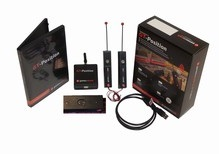
\includegraphics[scale=1.1]{figures/gotSystem.jpg} 
\caption{Games on Track GT-Position package [source:Games\ on\ Track]} 
\label{fig:GoTsystem}
\end{figure}
\noindent
%
The GoT software aggregates the received positions through time, and can be used to draw a map of the lawn, and to determine the absolute position of the tracked module.

GoT was originally designed for train modelling, but it is easily adaptable for any use of position tracking. In the following segment satellite based positioning systems are compared to the discussed GoT system.